\documentclass{standalone}
% translate with >> pdflatex -shell-escape <file>

% This file is an extract of the PGFPLOTS manual, copyright by Christian Feuersaenger.
% 
% Feel free to use it as long as you cite the pgfplots manual properly.
%
% See
%   http://pgfplots.sourceforge.net/pgfplots.pdf
% for the complete manual.
%
% Any required input files (for <plot table> or <plot file> or the table package) can be downloaded
% at
% http://www.ctan.org/tex-archive/graphics/pgf/contrib/pgfplots/doc/latex/
% and
% http://www.ctan.org/tex-archive/graphics/pgf/contrib/pgfplots/doc/latex/plotdata/

\usepackage{pgfplots}
\usepackage{pgfplotstable}
\pgfplotsset{compat=newest}

% The manual loads these libraries globally; the extracted standalone examples
% need them too. external/clickable/snakes are intentionally omitted.
\usetikzlibrary{
	arrows.meta,backgrounds,calc,decorations.footprints,decorations.markings,
	decorations.pathreplacing,fixedpointarithmetic,intersections,patterns,
	plotmarks,shapes.arrows,spy,through}
\usepgfplotslibrary{
	colorbrewer,colormaps,dateplot,fillbetween,groupplots,patchplots,polar,
	smithchart,statistics,ternary,units}

% Some colormap examples reuse this display style defined earlier in the manual.
\pgfplotsset{
	cycle from colormap manual style/.style={
		x=3cm,y=10pt,ytick=\empty,
		colorbar style={x=,y=,ytick=\empty},
		point meta min=0,point meta max=1,
		stack plots=y,
		y dir=reverse,colorbar style={y dir=reverse},
		every axis plot/.style={line width=2pt},
		legend entries={0,...,20},
		legend pos=outer north east,
	},
}

\pagestyle{empty}
\usetikzlibrary{spy}

\begin{document}
% requires \usetikzlibrary{spy}
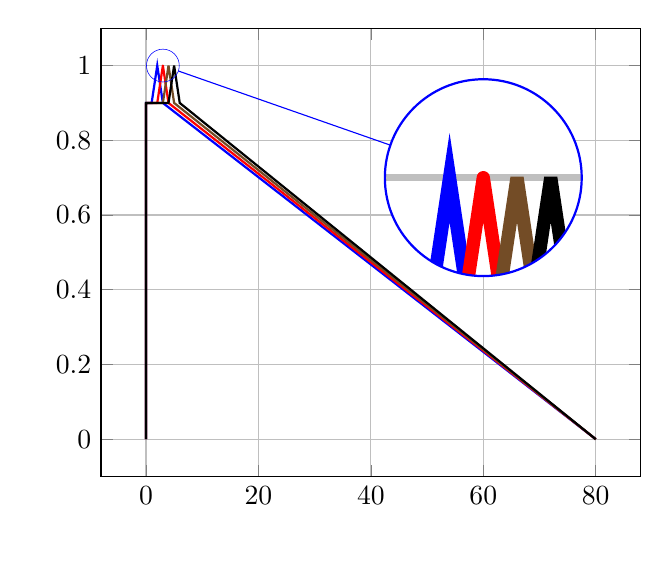
\begin{tikzpicture}[spy using outlines=
    {circle, magnification=6, connect spies}]
\begin{axis}[no markers,grid=major,
    every axis plot post/.append style={thick}]
\addplot  coordinates
 {(0, 0) (0, 0.9) (1, 0.9) (2, 1) (3, 0.9) (80, 0)};
\addplot+ [line join=round] coordinates
 {(0, 0) (0, 0.9) (2, 0.9) (3, 1) (4, 0.9) (80, 0)};
\addplot+ [line join=bevel] coordinates
 {(0, 0) (0, 0.9) (3, 0.9) (4, 1) (5, 0.9) (80, 0)};
\addplot+ [miter limit=5] coordinates
 {(0, 0) (0, 0.9) (4, 0.9) (5, 1) (6, 0.9) (80, 0)};

    \coordinate (spypoint)     at (3,1);
    \coordinate (magnifyglass) at (60,0.7);
\end{axis}

\spy [blue, size=2.5cm] on (spypoint)
    in node[fill=white] at (magnifyglass);
\end{tikzpicture}
\end{document}
